\documentclass[a4paper,12pt]{article}
\usepackage[utf8]{inputenc}
\usepackage[spanish]{babel}
\usepackage{graphicx}
\usepackage{amsmath}
\usepackage{booktabs}
\usepackage{hyperref}
\usepackage{geometry}
\geometry{margin=2.5cm}

\title{\texttt{Simulación de un Bot de Trading \\usando Eventos Discretos}}
\author{\\Darío López Falcón \\ Universidad de la Habana (UH) \\ Facultad de Matemática 
y Computación (MATCOM)}
\date{\today}

\begin{document}

\maketitle

\section*{S1. Introducción}

El presente proyecto tiene como objetivo desarrollar una simulación de eventos 
discretos para modelar el comportamiento de un bot de trading en un entorno de 
mercado simulado. Se busca analizar diferentes estrategias de compra y venta 
implementadas por bots con parámetros distintos, evaluando su desempeño bajo 
condiciones similares de volatilidad de precios.

El sistema simulado representa un mercado bursátil simplificado, en el cual el 
precio de un activo evoluciona a lo largo del tiempo según un modelo estocástico. 
Los bots toman decisiones en momentos discretos (cuando cambia el precio), por 
lo que el modelo se ajusta al paradigma de eventos discretos.

\textbf{Objetivos:}
\begin{itemize}
\item Modelar un entorno de mercado simulado con precios generados aleatoriamente.
\item Diseñar e implementar diferentes bots de trading basados en lógicas simples.
\item Evaluar el desempeño de los bots en términos de ganancia, número de operaciones y estabilidad.
\item Visualizar los resultados y analizar los factores que afectan el desempeño de cada estrategia.
\end{itemize}

\textbf{Variables de interés:} ganancia neta, cantidad de operaciones realizadas, 
valor final del portafolio, umbrales de compra y venta, comisión por transacción.

\section*{S2. Detalles de Implementación}

\textbf{Lenguaje:} Python 3.10

\textbf{Librerías principales:} numpy, matplotlib

\textbf{Estructura modular del código:}
\begin{itemize}
\item \texttt{main.py}: punto de entrada, controla la simulación.
\item \texttt{market.py}: generación de precios del activo usando ruido gaussiano.
\item \texttt{bot.py}: clase base de los bots con estrategias basadas en umbrales.
\item \texttt{simulator.py}: ejecución de la simulación, graficación y análisis visual.
\item \texttt{utils.py}: impresión de resumenes.
\end{itemize}

\textbf{Modelo de precios:} se generó una serie de precios a partir de un 
movimiento browniano simple:
\begin{equation*}
P_t = P_{t-1} + N(0, \sigma)
\end{equation*}

\textbf{Eventos simulados:} cada nuevo precio genera un evento donde los bots 
deciden si comprar, vender o mantener.

\textbf{Bots definidos:} se definieron múltiples bots con distintos umbrales de 
compra y venta, y comisiones por transacción. Las estrategias se mantienen 
simples para facilitar el análisis.

\section*{S3. Resultados y Experimentos}

A continuación se presenta la figura generada por la simulación, que incluye:
\begin{itemize}
\item Evolución del precio del activo.
\item Decisiones de compra (\textuparrow) y venta (\textdownarrow) de cada bot.
\item Cuadro comparativo con los parámetros y resultados de cada estrategia.
\end{itemize}

\begin{figure}[h!]
\centering
% 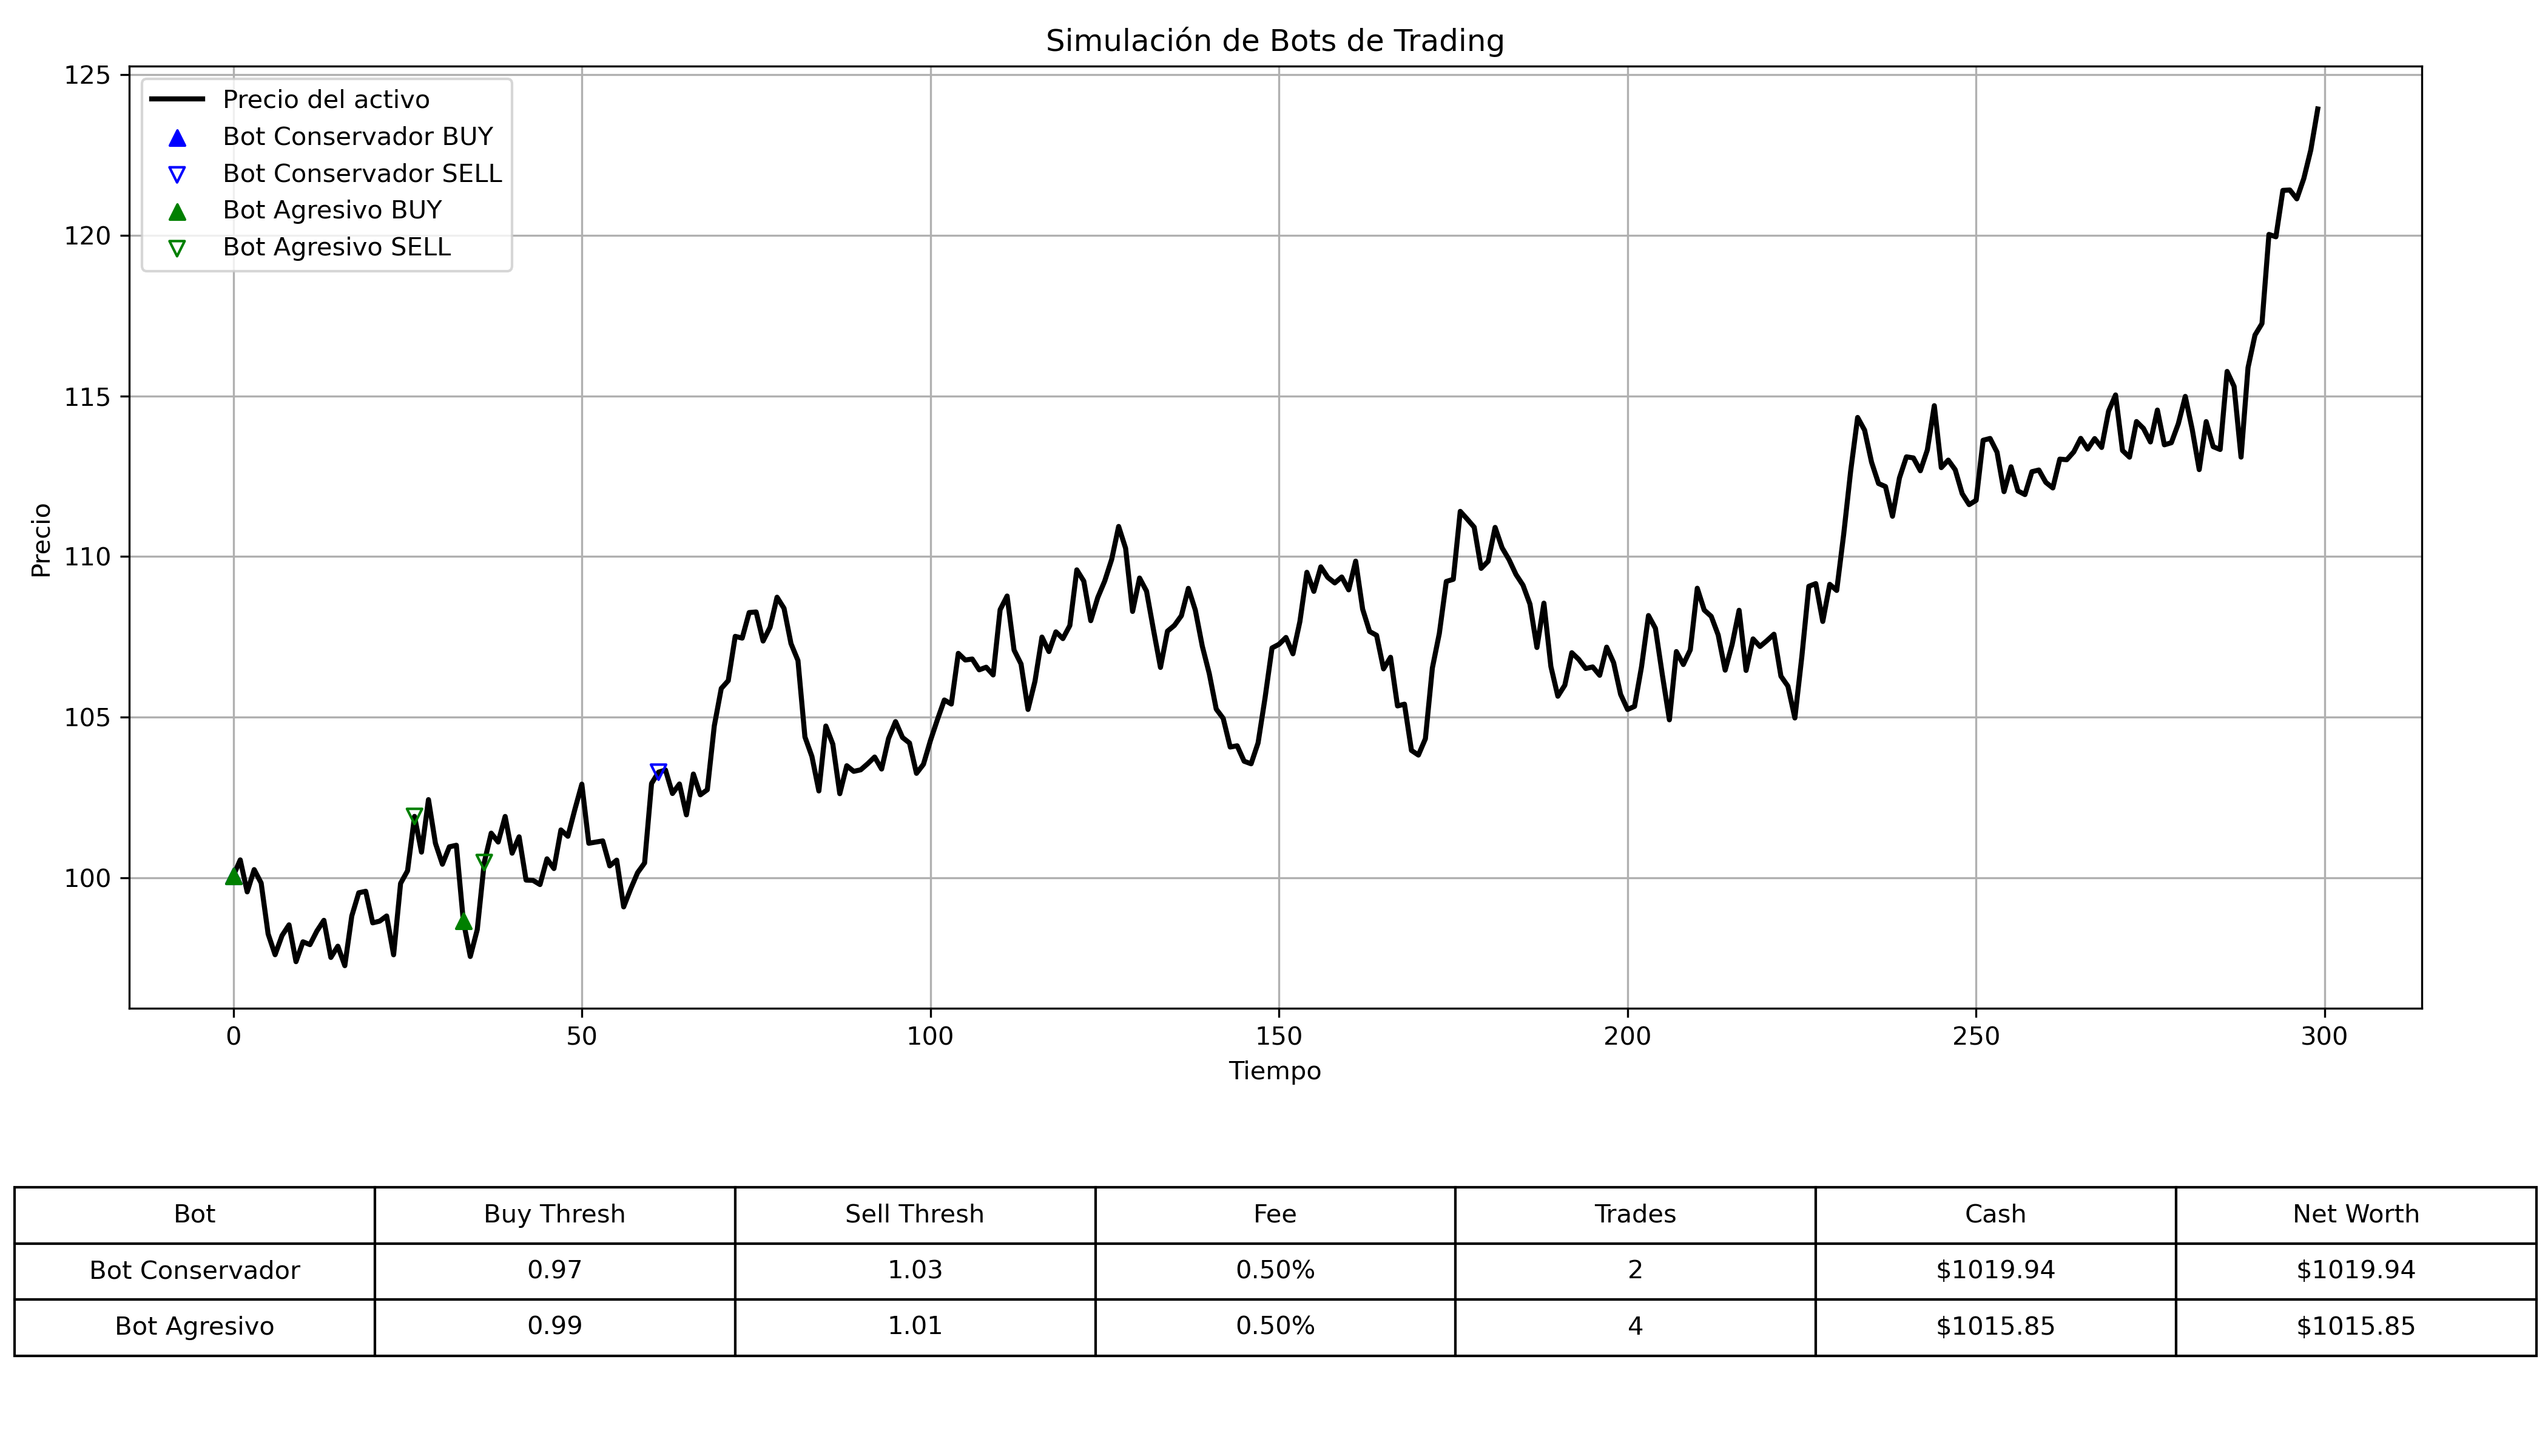
\includegraphics[width=0.95\textwidth]{figures/simulacion_trading.png}
\caption{Simulación de bots de trading sobre una serie de precios generados aleatoriamente.}
\end{figure}

\textbf{Hipótesis:}
\begin{itemize}
\item Los bots con umbrales más agresivos tienden a operar más, pero no necesariamente generan más ganancias.
\item Comisiones elevadas penalizan significativamente las estrategias con muchas operaciones.
\end{itemize}

\textbf{Observaciones:} se nota que el bot conservador realiza menos operaciones 
pero mantiene un valor de portafolio estable, mientras que el bot agresivo puede 
ganar más en ciertos escenarios pero también perder si hay oscilaciones rápidas 
del mercado.

\textbf{Análisis de parada:} se ejecutó la simulación por un número fijo de 
pasos. Para una versión más avanzada se podría implementar parada basada en 
convergencia de resultados o condiciones de mercado.

\section*{S4. Modelo Matemático (opcional)}

Se puede considerar como modelo subyacente un proceso estocástico de precios:
\begin{equation*}
\Delta P_t = N(0, \sigma^2)
\end{equation*}

Donde las decisiones de los bots se modelan como funciones deterministas sobre el estado actual:

\[\text{accion}(P_t) = 
    \begin{cases}  
        \text{comprar, si }P_t < P_{\text{compra}}\\
        \text{vender, si }P_t > P_{\text{venta}}\\
        \text{nada, eoc}
    \end{cases} 
\]

\section*{S5. Conclusiones}

Este trabajo demuestra que la simulación de eventos discretos es una herramienta 
versátil para evaluar estrategias de trading en mercados simplificados. Aunque 
los modelos son sencillos, permiten experimentar con lógicas de decisión y 
observar sus efectos en un entorno controlado.

La extensión de este trabajo podría incluir:
\begin{itemize}
\item Incorporación de datos reales de mercado.
\item Modelos de precios más realistas (ej.\ procesos de Lévy, GARCH).
\item Estrategias de bots con aprendizaje automático.
\item Simulación multiagente con bots competidores.
\end{itemize}

\end{document}
